\documentclass[9pt,letterpaper]{article}
%\usepackage[utf8]{inputenc}
\UseRawInputEncoding
\usepackage[english]{babel}
\usepackage{listings}
\usepackage{xcolor}
\usepackage{graphicx}

%For syntax highlighting
\definecolor{codegreen}{rgb}{0,0.6,0}
\definecolor{codegray}{rgb}{0.5,0.5,0.5}
\definecolor{codepurple}{rgb}{0.58,0,0.82}
\definecolor{backcolour}{rgb}{1,1,1}

%%Sets different parameters
\lstdefinestyle{mystyle}{
    backgroundcolor=\color{backcolour},   
    commentstyle=\color{codegreen},
    keywordstyle=\color{magenta},
    numberstyle=\tiny\color{codegray},
    stringstyle=\color{codepurple},
    basicstyle=\ttfamily\footnotesize,
    breakatwhitespace=false,         
    breaklines=true,                 
    captionpos=b,                    
    keepspaces=true,                 
    numbers=left,                    
    numbersep=5pt,                  
    showspaces=false,                
    showstringspaces=false,
    showtabs=false,                  
    tabsize=4
}
\lstset{style=mystyle}

\title{\textbf{Department of Computer Science and Engineering}}
\author{\textbf{Shivanirudh S G, 185001146, Semester VII }}

\date{27 August 2021}

\begin{document}
\maketitle
\hrule
\section*{\center{UCS1712 - Graphics and Multimedia Lab}}
\hrule 
\bigskip\bigskip

%Assignment name
\subsection*{\center{\textbf{Exercise 6: 2D Composite Transformations and Windowing in C++ using OpenGL}}}

%Objective
\subsection*{\flushleft{Aim:}}
\begin{flushleft}
     To compute the composite transformation matrix for any 2 transformations given as input by the user and applying it on the object.
\end{flushleft}

%Code
\subsection*{\flushleft{Code:}}
\begin{flushleft}
\lstinputlisting[language = C++]{CompositeTransformations/Headers.h}
\lstinputlisting[language = C++]{CompositeTransformations/Signatures.h}
\lstinputlisting[language = C++]{CompositeTransformations/Helpers.h}
\lstinputlisting[language = C++]{CompositeTransformations/main.cpp}
\end{flushleft}
\newpage
\subsection*{\flushleft{Output:}}
\textbf{Original Image:}\\
Choose number of edges: (1 for line, 3 and upwards for polygon): 5\\
Enter vertices:\\ 
Vertex 1 (x,y): 30 30\\
Vertex 2 (x,y): 10 60\\
Vertex 3 (x,y): 60 80\\
Vertex 4 (x,y): 110 60\\
Vertex 5 (x,y): 90 30\\
Number of edges: 5\\
\begin{figure}[h]
    \centering
    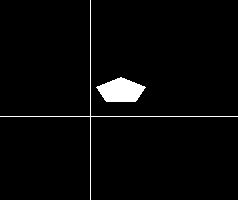
\includegraphics[height=5cm]{CompositeTransformations/Outputs/Original.png}
\end{figure}

%---------------------------------------------------------------------------------------------------------
\newpage
\textbf{\Large{First transform: Translation}}

Choose first transformation: \\
1 for Translation\\
2 for Rotation\\
3 for Scaling\\
4 for Reflection\\
5 for shearing\\
0 to Exit\\
Enter your choice: 1\\
\\
Enter the translation factor for X and Y: 40 40\\


\textbf{\large{Second Transform: Rotation}}\\
Enter the rotation angle: 90   \\
Enter point about which to be rotated: 0 0\\

\begin{figure}[h]
    \centering
    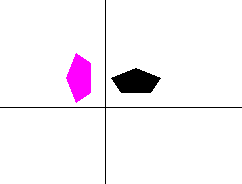
\includegraphics[height=5cm]{CompositeTransformations/Outputs/TranslateRotate.png}
\end{figure}

\newpage

\textbf{\large{Second Transform: Scaling}}\\
Enter the scaling factor for X and Y: 3 3\\
Enter point about which to be scaled: 0 0\\

\begin{figure}[h]
    \centering
    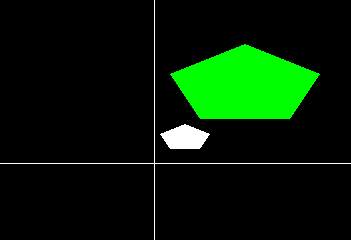
\includegraphics[height=5cm]{CompositeTransformations/Outputs/TranslateScale.png}
\end{figure}

\textbf{\large{Second Transform: Reflection}}\\
Enter the angle with X-axis and Y-intercept of the mirror: 90 0\\

\begin{figure}[h]
    \centering
    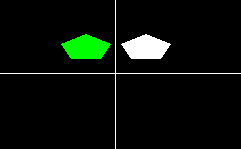
\includegraphics[height=5cm]{CompositeTransformations/Outputs/TranslateReflect.png}
\end{figure}

\newpage

\textbf{\large{Second Transform: Shearing}}\\
Enter the shearing factor for X and Y: 3 3 \\

\begin{figure}[h]
    \centering
    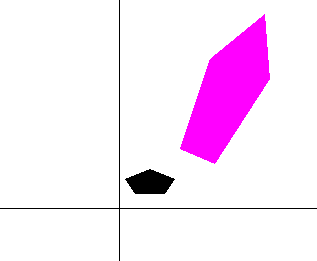
\includegraphics[height=5cm]{CompositeTransformations/Outputs/TranslateShear.png}
\end{figure}

\newpage
%---------------------------------------------------------------------------------------------------------
\textbf{\Large{First transform: Rotation}}

Choose first transformation: \\
1 for Translation\\
2 for Rotation\\
3 for Scaling\\
4 for Reflection\\
5 for shearing\\
0 to Exit\\
Enter your choice: 2\\
Enter the rotation angle: 45\\
Enter point about which to be rotated: 0 0\\


\textbf{\large{Second Transform: Translation}}\\
Enter the translation factor for X and Y: 50 50 \\

\begin{figure}[h]
    \centering
    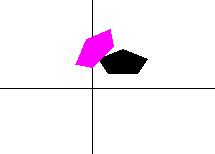
\includegraphics[height=5cm]{CompositeTransformations/Outputs/RotateTranslate.png}
\end{figure}

\newpage

\textbf{\large{Second Transform: Scaling}}\\
Enter the scaling factor for X and Y: 3 3\\
Enter point about which to be scaled: 0 0\\

\begin{figure}[h]
    \centering
    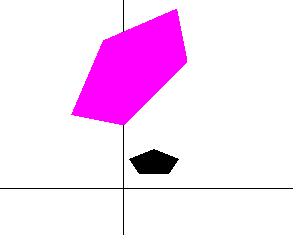
\includegraphics[height=5cm]{CompositeTransformations/Outputs/RotateScale.png}
\end{figure}

\textbf{\large{Second Transform: Reflection}}\\
Enter the angle with X-axis and Y-intercept of the mirror: 0 0\\

\begin{figure}[h]
    \centering
    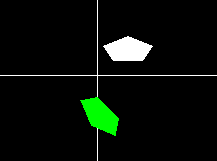
\includegraphics[height=5cm]{CompositeTransformations/Outputs/RotateReflect.png}
\end{figure}

\newpage

\textbf{\large{Second Transform: Shearing}}\\
Enter the shearing factor for X and Y: 3 3 \\

\begin{figure}[h]
    \centering
    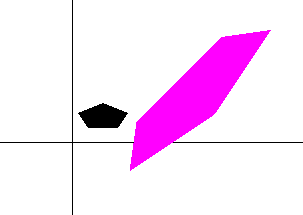
\includegraphics[height=5cm]{CompositeTransformations/Outputs/RotateShear.png}
\end{figure}

\newpage
%---------------------------------------------------------------------------------------------------------

\textbf{\Large{First transform: Scaling }}

Choose first transformation: \\
1 for Translation\\
2 for Rotation\\
3 for Scaling\\
4 for Reflection\\
5 for shearing\\
0 to Exit\\
Enter your choice: 3\\
Enter the scaling factor for X and Y: 3 3\\
Enter point about which to be scaled: 0 0\\


\textbf{\large{Second Transform: Translation}}\\
Enter the translation factor for X and Y: 50 50 \\

\begin{figure}[h]
    \centering
    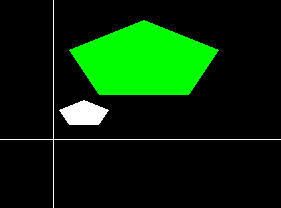
\includegraphics[height=5cm]{CompositeTransformations/Outputs/ScaleTranslate.png}
\end{figure}

\newpage

\textbf{\large{Second Transform: Rotation}}\\
Enter the rotation angle: 45 \\
Enter point about which to be rotated: 0 0\\

\begin{figure}[h]
    \centering
    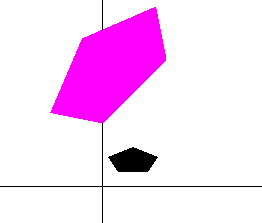
\includegraphics[height=5cm]{CompositeTransformations/Outputs/ScaleRotate.png}
\end{figure}

\textbf{\large{Second Transform: Reflection}}\\
Enter the angle with X-axis and Y-intercept of the mirror: 135 0\\

\begin{figure}[h]
    \centering
    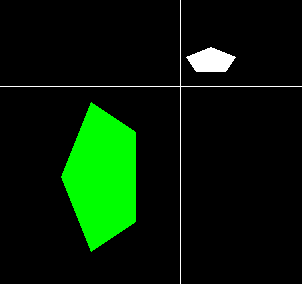
\includegraphics[height=5cm]{CompositeTransformations/Outputs/ScaleReflect.png}
\end{figure}

\newpage

\textbf{\large{Second Transform: Shearing}}\\
Enter the shearing factor for X and Y: 0.5 0.5 \\

\begin{figure}[h]
    \centering
    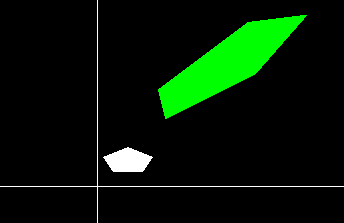
\includegraphics[height=5cm]{CompositeTransformations/Outputs/ScaleShear.png}
\end{figure}

\newpage

\textbf{\Large{First transform: Reflecttion}}

Choose first transformation: \\
1 for Translation\\
2 for Rotation\\
3 for Scaling\\
4 for Reflection\\
5 for shearing\\
0 to Exit\\
Enter your choice: 4\\
Enter the angle with X-axis and Y-intercept of the mirror: 0 0\\


\textbf{\large{Second Transform: Translation}}\\
Enter the translation factor for X and Y: 50 50 \\

\begin{figure}[h]
    \centering
    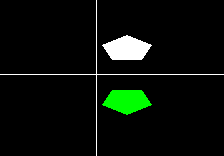
\includegraphics[height=5cm]{CompositeTransformations/Outputs/ReflectTranslate.png}
\end{figure}

\newpage

\textbf{\large{Second Transform: Rotation}}\\
Enter the rotation angle: 90 \\
Enter point about which to be rotated: 0 0\\

\begin{figure}[h]
    \centering
    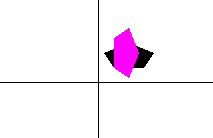
\includegraphics[height=5cm]{CompositeTransformations/Outputs/ReflectRotate.png}
\end{figure}

\textbf{\large{Second Transform: Scaling}}\\
Enter the scaling factor for X and Y: 3 3\\
Enter point about which to be scaled: 0 0\\

\begin{figure}[h]
    \centering
    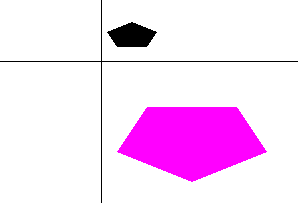
\includegraphics[height=5cm]{CompositeTransformations/Outputs/ReflectScale.png}
\end{figure}

\newpage

\textbf{\large{Second Transform: Shearing}}\\
Enter the shearing factor for X and Y: 3 3 \\

\begin{figure}[h]
    \centering
    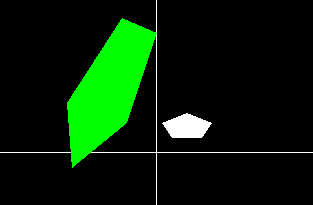
\includegraphics[height=5cm]{CompositeTransformations/Outputs/ReflectShear.png}
\end{figure}

\newpage

\textbf{\Large{First transform: Shearing}}

Choose first transformation: \\
1 for Translation\\
2 for Rotation\\
3 for Scaling\\
4 for Reflection\\
5 for shearing\\
0 to Exit\\
Enter your choice: 5\\
Enter the shearing factor for X and Y: 0.5 0.5\\


\textbf{\large{Second Transform: Translation}}\\
Enter the translation factor for X and Y: 40 40 \\

\begin{figure}[h]
    \centering
    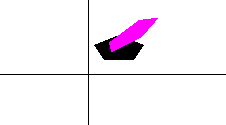
\includegraphics[height=5cm]{CompositeTransformations/Outputs/ShearTranslate.png}
\end{figure}

\newpage

\textbf{\large{Second Transform: Rotation}}
Enter the rotation angle: 90\\
Enter point about which to be rotated: 0 0\\

\begin{figure}[h]
    \centering
    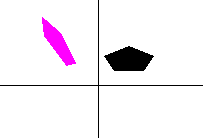
\includegraphics[height=5cm]{CompositeTransformations/Outputs/ShearRotate.png}
\end{figure}

\textbf{\large{Second Transform: Scaling}}\\
Enter the scaling factor for X and Y: 3 3\\
Enter point about which to be scaled: 0 0\\

\begin{figure}[h]
    \centering
    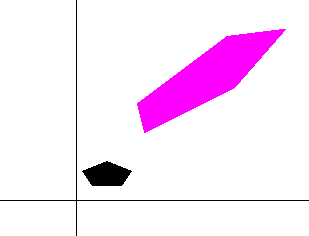
\includegraphics[height=5cm]{CompositeTransformations/Outputs/ShearScale.png}
\end{figure}

\newpage

\textbf{\large{Second Transform: Reflection}}\\
Enter the angle with X-axis and Y-intercept of the mirror: 0 0\\

\begin{figure}[h]
    \centering
    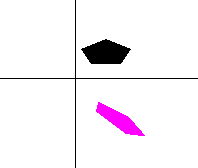
\includegraphics[height=5cm]{CompositeTransformations/Outputs/ShearReflect.png}
\end{figure}

\newpage

\bigskip\bigskip
\hrule

\subsection*{\flushleft{Aim:}}
\begin{flushleft}
     Create a window with any 2D object and a different sized viewport. Apply window to viewport transformation on the object. Display both window and viewport.
\end{flushleft}

%Code
\subsection*{\flushleft{Code:}}
\begin{flushleft}
\lstinputlisting[language = C++]{Windowing/Headers.h}
\lstinputlisting[language = C++]{Windowing/Signatures.h}
\lstinputlisting[language = C++]{Windowing/Helpers.h}
\lstinputlisting[language = C++]{Windowing/main.cpp}
\end{flushleft}
\newpage
\subsection*{\flushleft{Output:}}

Enter window dimensions: \\
Enter minimum X value: 50\\
Enter maximum X value: 250\\
Enter minimum Y value: 50\\
Enter maximum Y value: 250\\

Choose number of edges: (1 for line, 3 and upwards for polygon): 5\\
Enter vertices: \\
Vertex 1 (x,y): 80 80 \\
Vertex 2 (x,y): 60 110\\
Vertex 3 (x,y): 110 130\\
Vertex 4 (x,y): 160 110\\
Vertex 5 (x,y): 140 80\\

Enter viewport dimensions:\\ 
Enter minimum X value: 50 \\
Enter maximum X value: 100\\
Enter minimum Y value: 300\\
Enter maximum Y value: 350\\

\begin{figure}[h]
    \centering
    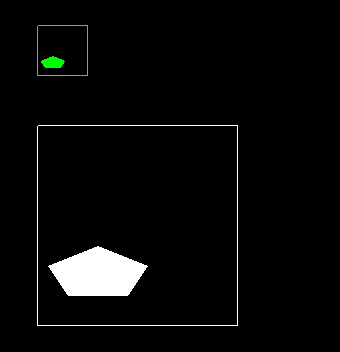
\includegraphics[height=5cm]{Windowing/Outputs/Windowing.png}
\end{figure}

\bigskip\bigskip
\hrule

\end{document}